% Options for packages loaded elsewhere
\PassOptionsToPackage{unicode}{hyperref}
\PassOptionsToPackage{hyphens}{url}
\PassOptionsToPackage{dvipsnames,svgnames,x11names}{xcolor}
%
\documentclass[
  letterpaper,
  DIV=11,
  numbers=noendperiod]{scrartcl}

\usepackage{amsmath,amssymb}
\usepackage{iftex}
\ifPDFTeX
  \usepackage[T1]{fontenc}
  \usepackage[utf8]{inputenc}
  \usepackage{textcomp} % provide euro and other symbols
\else % if luatex or xetex
  \usepackage{unicode-math}
  \defaultfontfeatures{Scale=MatchLowercase}
  \defaultfontfeatures[\rmfamily]{Ligatures=TeX,Scale=1}
\fi
\usepackage{lmodern}
\ifPDFTeX\else  
    % xetex/luatex font selection
\fi
% Use upquote if available, for straight quotes in verbatim environments
\IfFileExists{upquote.sty}{\usepackage{upquote}}{}
\IfFileExists{microtype.sty}{% use microtype if available
  \usepackage[]{microtype}
  \UseMicrotypeSet[protrusion]{basicmath} % disable protrusion for tt fonts
}{}
\makeatletter
\@ifundefined{KOMAClassName}{% if non-KOMA class
  \IfFileExists{parskip.sty}{%
    \usepackage{parskip}
  }{% else
    \setlength{\parindent}{0pt}
    \setlength{\parskip}{6pt plus 2pt minus 1pt}}
}{% if KOMA class
  \KOMAoptions{parskip=half}}
\makeatother
\usepackage{xcolor}
\setlength{\emergencystretch}{3em} % prevent overfull lines
\setcounter{secnumdepth}{-\maxdimen} % remove section numbering
% Make \paragraph and \subparagraph free-standing
\ifx\paragraph\undefined\else
  \let\oldparagraph\paragraph
  \renewcommand{\paragraph}[1]{\oldparagraph{#1}\mbox{}}
\fi
\ifx\subparagraph\undefined\else
  \let\oldsubparagraph\subparagraph
  \renewcommand{\subparagraph}[1]{\oldsubparagraph{#1}\mbox{}}
\fi

\usepackage{color}
\usepackage{fancyvrb}
\newcommand{\VerbBar}{|}
\newcommand{\VERB}{\Verb[commandchars=\\\{\}]}
\DefineVerbatimEnvironment{Highlighting}{Verbatim}{commandchars=\\\{\}}
% Add ',fontsize=\small' for more characters per line
\usepackage{framed}
\definecolor{shadecolor}{RGB}{241,243,245}
\newenvironment{Shaded}{\begin{snugshade}}{\end{snugshade}}
\newcommand{\AlertTok}[1]{\textcolor[rgb]{0.68,0.00,0.00}{#1}}
\newcommand{\AnnotationTok}[1]{\textcolor[rgb]{0.37,0.37,0.37}{#1}}
\newcommand{\AttributeTok}[1]{\textcolor[rgb]{0.40,0.45,0.13}{#1}}
\newcommand{\BaseNTok}[1]{\textcolor[rgb]{0.68,0.00,0.00}{#1}}
\newcommand{\BuiltInTok}[1]{\textcolor[rgb]{0.00,0.23,0.31}{#1}}
\newcommand{\CharTok}[1]{\textcolor[rgb]{0.13,0.47,0.30}{#1}}
\newcommand{\CommentTok}[1]{\textcolor[rgb]{0.37,0.37,0.37}{#1}}
\newcommand{\CommentVarTok}[1]{\textcolor[rgb]{0.37,0.37,0.37}{\textit{#1}}}
\newcommand{\ConstantTok}[1]{\textcolor[rgb]{0.56,0.35,0.01}{#1}}
\newcommand{\ControlFlowTok}[1]{\textcolor[rgb]{0.00,0.23,0.31}{#1}}
\newcommand{\DataTypeTok}[1]{\textcolor[rgb]{0.68,0.00,0.00}{#1}}
\newcommand{\DecValTok}[1]{\textcolor[rgb]{0.68,0.00,0.00}{#1}}
\newcommand{\DocumentationTok}[1]{\textcolor[rgb]{0.37,0.37,0.37}{\textit{#1}}}
\newcommand{\ErrorTok}[1]{\textcolor[rgb]{0.68,0.00,0.00}{#1}}
\newcommand{\ExtensionTok}[1]{\textcolor[rgb]{0.00,0.23,0.31}{#1}}
\newcommand{\FloatTok}[1]{\textcolor[rgb]{0.68,0.00,0.00}{#1}}
\newcommand{\FunctionTok}[1]{\textcolor[rgb]{0.28,0.35,0.67}{#1}}
\newcommand{\ImportTok}[1]{\textcolor[rgb]{0.00,0.46,0.62}{#1}}
\newcommand{\InformationTok}[1]{\textcolor[rgb]{0.37,0.37,0.37}{#1}}
\newcommand{\KeywordTok}[1]{\textcolor[rgb]{0.00,0.23,0.31}{#1}}
\newcommand{\NormalTok}[1]{\textcolor[rgb]{0.00,0.23,0.31}{#1}}
\newcommand{\OperatorTok}[1]{\textcolor[rgb]{0.37,0.37,0.37}{#1}}
\newcommand{\OtherTok}[1]{\textcolor[rgb]{0.00,0.23,0.31}{#1}}
\newcommand{\PreprocessorTok}[1]{\textcolor[rgb]{0.68,0.00,0.00}{#1}}
\newcommand{\RegionMarkerTok}[1]{\textcolor[rgb]{0.00,0.23,0.31}{#1}}
\newcommand{\SpecialCharTok}[1]{\textcolor[rgb]{0.37,0.37,0.37}{#1}}
\newcommand{\SpecialStringTok}[1]{\textcolor[rgb]{0.13,0.47,0.30}{#1}}
\newcommand{\StringTok}[1]{\textcolor[rgb]{0.13,0.47,0.30}{#1}}
\newcommand{\VariableTok}[1]{\textcolor[rgb]{0.07,0.07,0.07}{#1}}
\newcommand{\VerbatimStringTok}[1]{\textcolor[rgb]{0.13,0.47,0.30}{#1}}
\newcommand{\WarningTok}[1]{\textcolor[rgb]{0.37,0.37,0.37}{\textit{#1}}}

\providecommand{\tightlist}{%
  \setlength{\itemsep}{0pt}\setlength{\parskip}{0pt}}\usepackage{longtable,booktabs,array}
\usepackage{calc} % for calculating minipage widths
% Correct order of tables after \paragraph or \subparagraph
\usepackage{etoolbox}
\makeatletter
\patchcmd\longtable{\par}{\if@noskipsec\mbox{}\fi\par}{}{}
\makeatother
% Allow footnotes in longtable head/foot
\IfFileExists{footnotehyper.sty}{\usepackage{footnotehyper}}{\usepackage{footnote}}
\makesavenoteenv{longtable}
\usepackage{graphicx}
\makeatletter
\def\maxwidth{\ifdim\Gin@nat@width>\linewidth\linewidth\else\Gin@nat@width\fi}
\def\maxheight{\ifdim\Gin@nat@height>\textheight\textheight\else\Gin@nat@height\fi}
\makeatother
% Scale images if necessary, so that they will not overflow the page
% margins by default, and it is still possible to overwrite the defaults
% using explicit options in \includegraphics[width, height, ...]{}
\setkeys{Gin}{width=\maxwidth,height=\maxheight,keepaspectratio}
% Set default figure placement to htbp
\makeatletter
\def\fps@figure{htbp}
\makeatother

\KOMAoption{captions}{tableheading}
\makeatletter
\makeatother
\makeatletter
\makeatother
\makeatletter
\@ifpackageloaded{caption}{}{\usepackage{caption}}
\AtBeginDocument{%
\ifdefined\contentsname
  \renewcommand*\contentsname{Table of contents}
\else
  \newcommand\contentsname{Table of contents}
\fi
\ifdefined\listfigurename
  \renewcommand*\listfigurename{List of Figures}
\else
  \newcommand\listfigurename{List of Figures}
\fi
\ifdefined\listtablename
  \renewcommand*\listtablename{List of Tables}
\else
  \newcommand\listtablename{List of Tables}
\fi
\ifdefined\figurename
  \renewcommand*\figurename{Figure}
\else
  \newcommand\figurename{Figure}
\fi
\ifdefined\tablename
  \renewcommand*\tablename{Table}
\else
  \newcommand\tablename{Table}
\fi
}
\@ifpackageloaded{float}{}{\usepackage{float}}
\floatstyle{ruled}
\@ifundefined{c@chapter}{\newfloat{codelisting}{h}{lop}}{\newfloat{codelisting}{h}{lop}[chapter]}
\floatname{codelisting}{Listing}
\newcommand*\listoflistings{\listof{codelisting}{List of Listings}}
\makeatother
\makeatletter
\@ifpackageloaded{caption}{}{\usepackage{caption}}
\@ifpackageloaded{subcaption}{}{\usepackage{subcaption}}
\makeatother
\makeatletter
\@ifpackageloaded{tcolorbox}{}{\usepackage[skins,breakable]{tcolorbox}}
\makeatother
\makeatletter
\@ifundefined{shadecolor}{\definecolor{shadecolor}{rgb}{.97, .97, .97}}
\makeatother
\makeatletter
\makeatother
\makeatletter
\makeatother
\ifLuaTeX
  \usepackage{selnolig}  % disable illegal ligatures
\fi
\IfFileExists{bookmark.sty}{\usepackage{bookmark}}{\usepackage{hyperref}}
\IfFileExists{xurl.sty}{\usepackage{xurl}}{} % add URL line breaks if available
\urlstyle{same} % disable monospaced font for URLs
\hypersetup{
  pdftitle={Introducing CanvasXpress for Python!},
  colorlinks=true,
  linkcolor={blue},
  filecolor={Maroon},
  citecolor={Blue},
  urlcolor={Blue},
  pdfcreator={LaTeX via pandoc}}

\title{Introducing CanvasXpress for Python!}
\author{}
\date{}

\begin{document}
\maketitle
\ifdefined\Shaded\renewenvironment{Shaded}{\begin{tcolorbox}[sharp corners, breakable, interior hidden, frame hidden, borderline west={3pt}{0pt}{shadecolor}, boxrule=0pt, enhanced]}{\end{tcolorbox}}\fi

\hypertarget{a-high-performance-plotting-library}{%
\subsection{A High Performance Plotting
Library}\label{a-high-performance-plotting-library}}

I'm pleased to introduce
\href{https://pypi.org/project/canvasxpress/}{CanvasXpress for Python}:
an extension to the highly performant
\href{https://canvasxpress.org}{JavaScript Library} developed by
Dr.~Isaac Nuehaus for producing chart illustrations and facilitating
data exploration.

Scientific computing often requires that very large data sets be
visualized to facilitate analysis and research. Unfortunately, most
modern charting libraries for Web browsers use methods that cannot
efficiently illustrate, if even at all, data sets larger than a few
thousand data points. CanvasXpress, which was originally developed as
the core visualization component for bioinformatics and systems biology
at Bristol-Myers Squibb, uses a very different approach to rendering
that enables it to produce beautiful, interactive illustrations at
scale---for example, million-point heat maps. CanvasXpress does this for
a rich variety of chart types, examples of which are presented here:

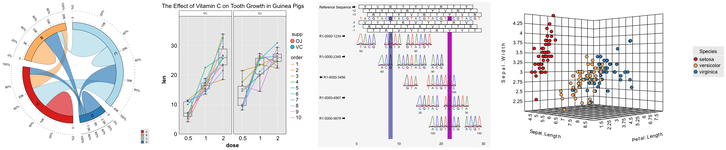
\includegraphics{sample_graphs.png}

Upon being rendered in a Web environment, the charts can then be
explored in detail using a variety of tools. The user can use menu and
configuration tools to review the data table; segregate or group data
fields; shape or color points based on primary or meta properties; or
even re-illustrate the chart altogether, such as changing a bar chart
into a tree map. Many of these exploration features would normally
require the use of standalone and potentially expensive applications,
such as Tableau, but CanvasXpress treats interactive data review as a
first-class feature standard in every chart. Here is a dashboard chart
with its data table and configuration tools presented:

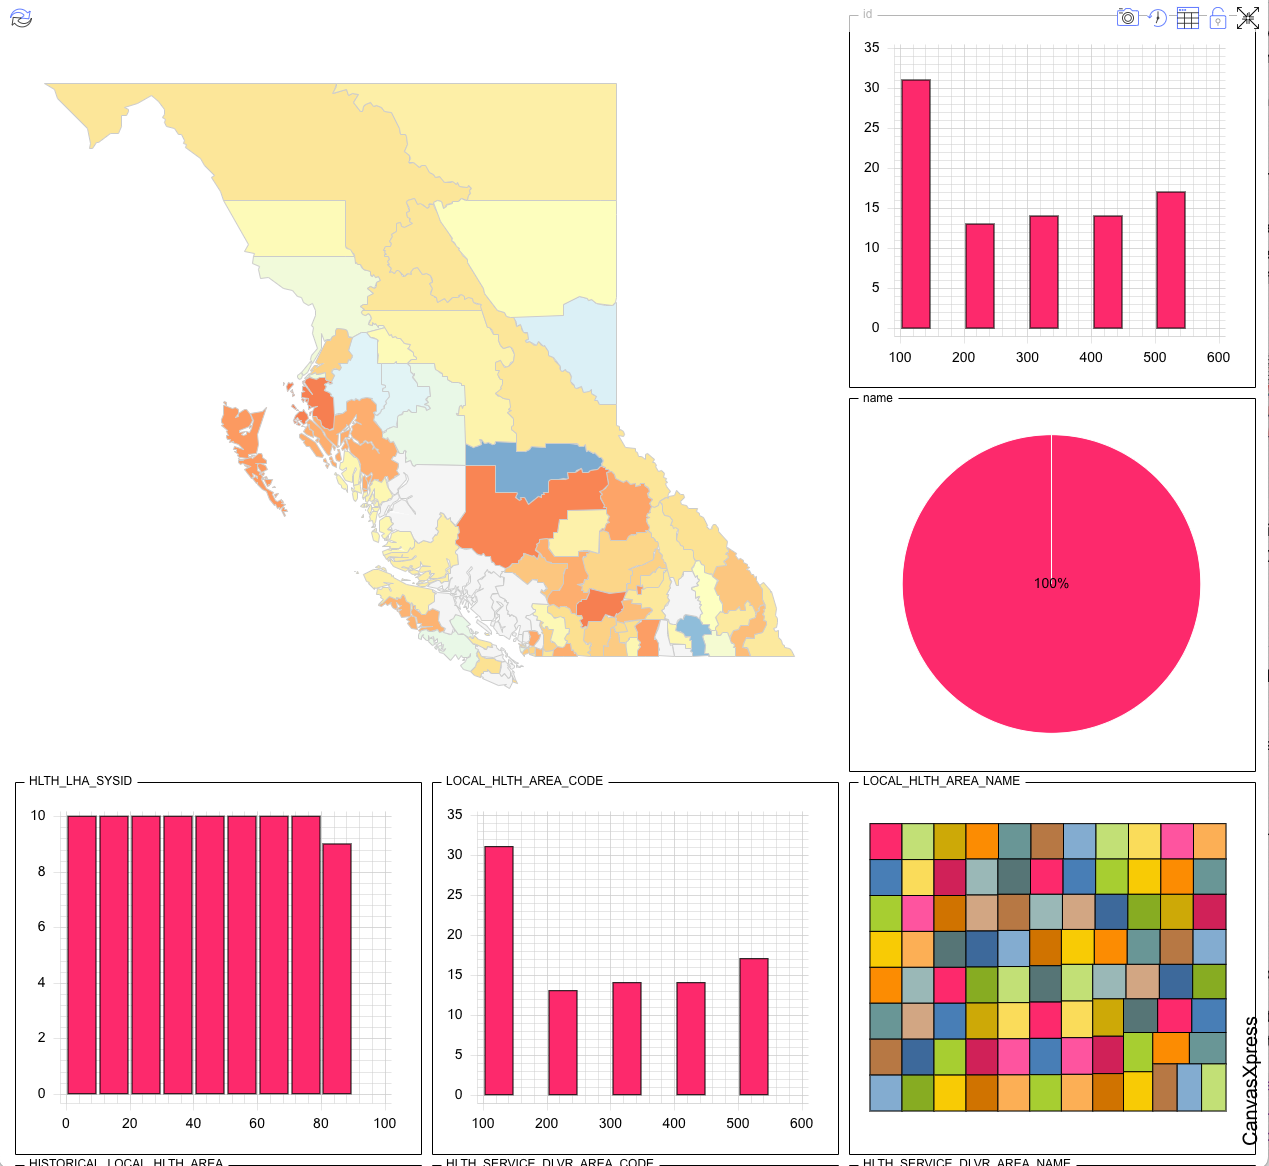
\includegraphics[width=2.86458in,height=\textheight]{dashboard_chart.png}
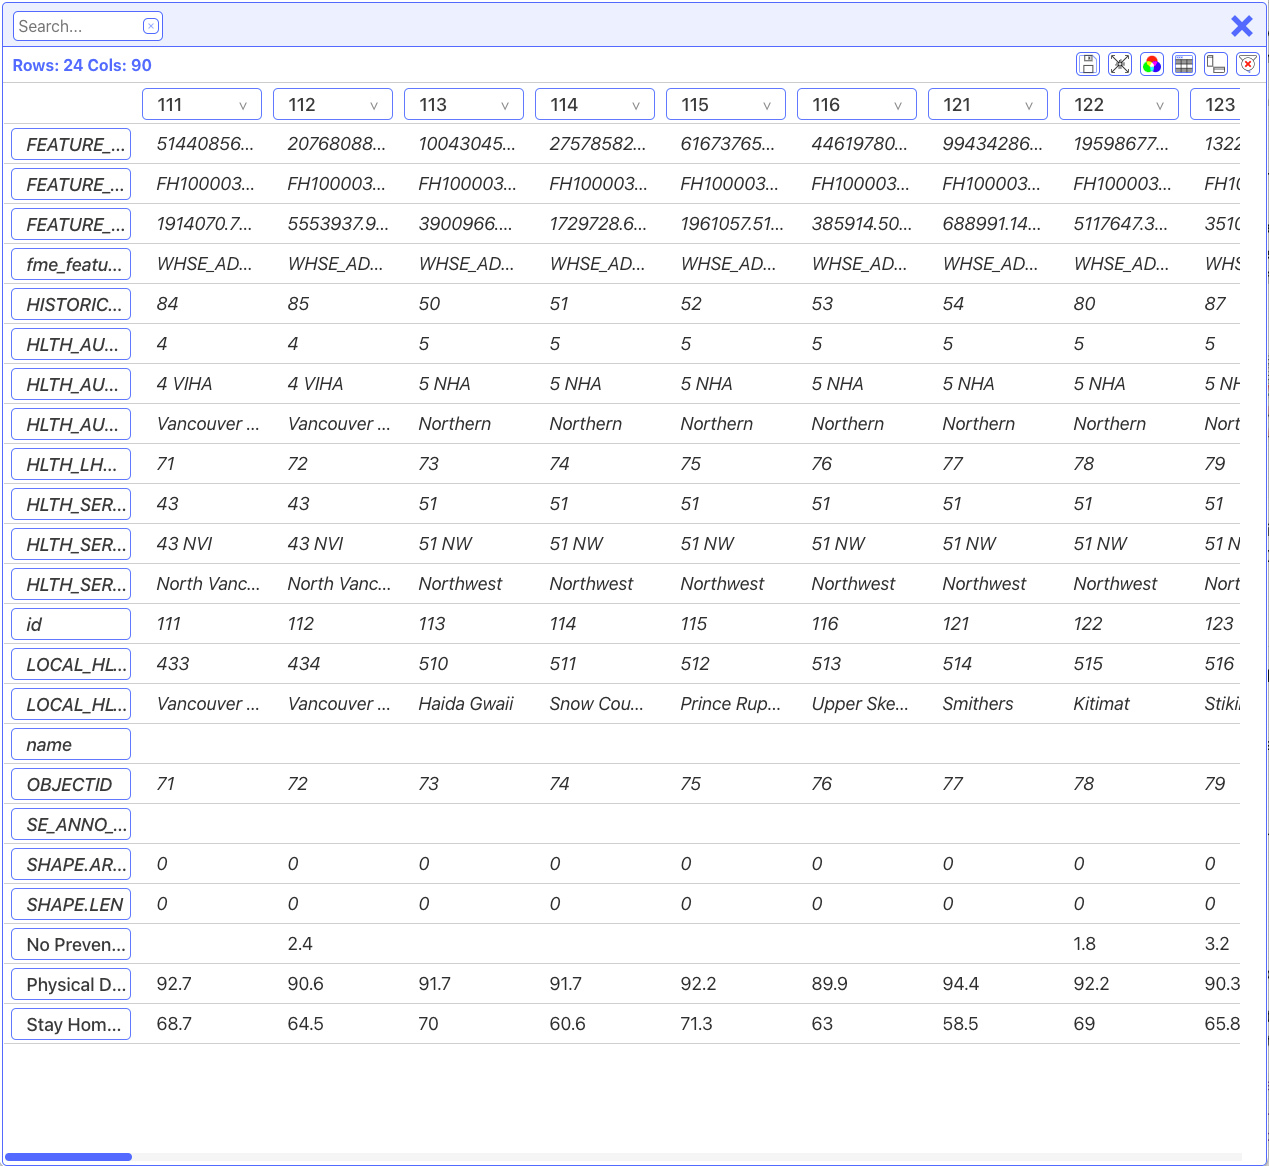
\includegraphics[width=2.86458in,height=\textheight]{dashboard_data.png}
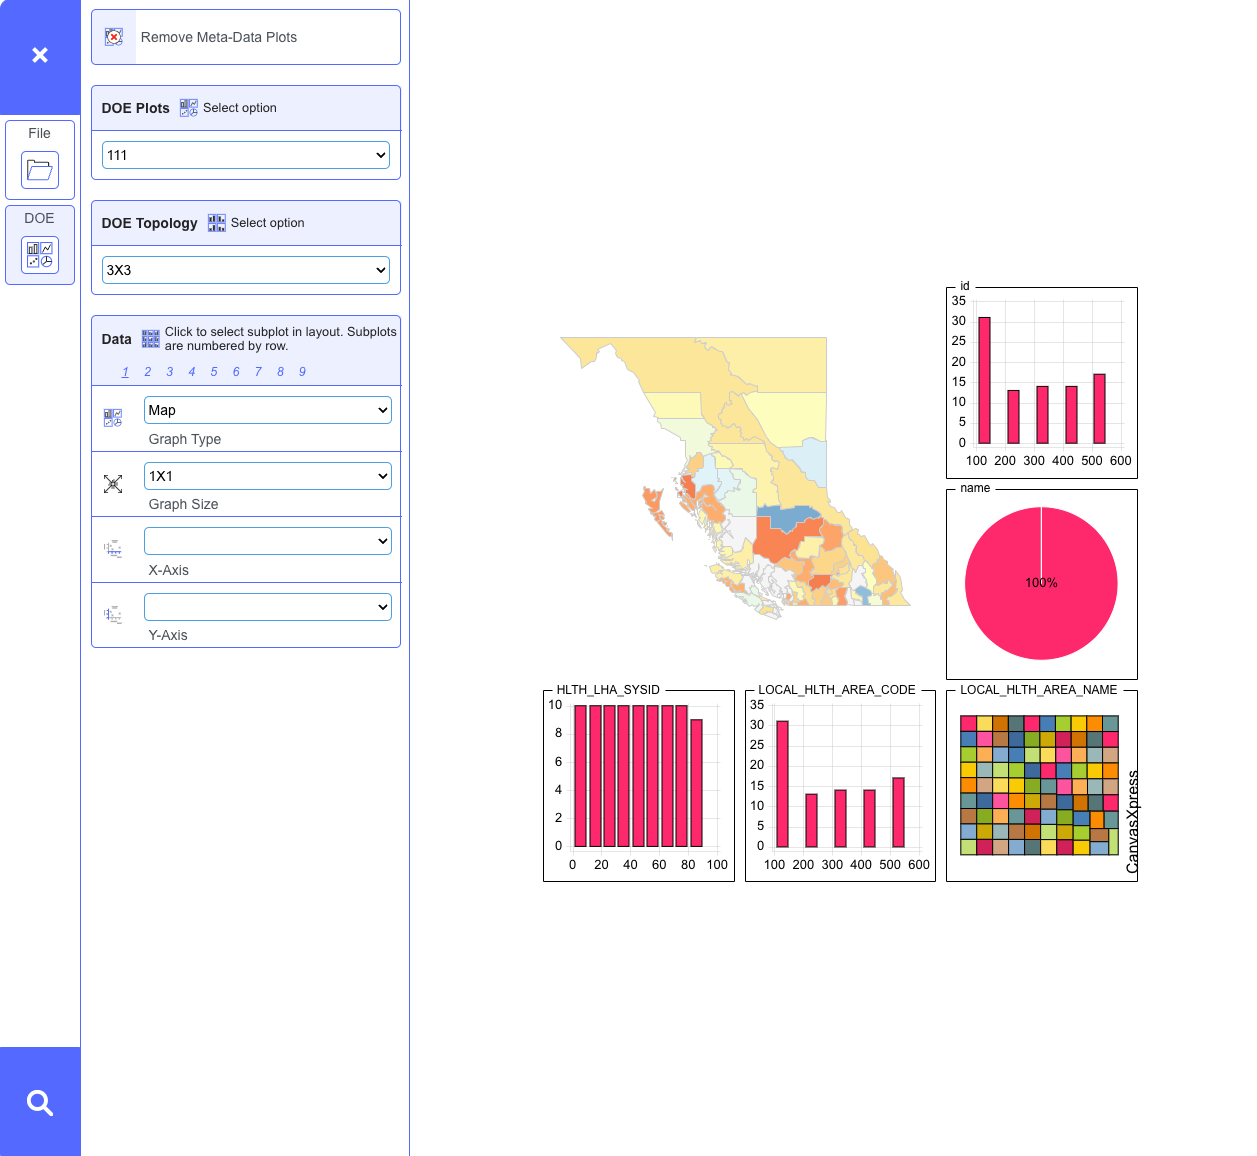
\includegraphics[width=2.86458in,height=\textheight]{dashboard_config.png}

Not only can each chart be explored in detail, but charts on the same
page broadcast changes to their peers. For example, if two or more
charts on the same page use the same data set then data selection in one
chart will update peers so that the same data is selected in the other
charts---even if the types of charts are different. This is a powerful
means by which complex data analysis can be facilitated by breaking
complex data into simpler charts that better highlight related but
illustratively unique data characteristics from the overall set.

\hypertarget{platform-native-approaches}{%
\subsection{Platform Native
Approaches}\label{platform-native-approaches}}

Our company, \href{https://www.aggregate-genius.com/}{Aggregate Genius
Inc.} specializes in custom analytics solutions for the scientific and
business communities, and of course visualizations for complex data is a
key part of our work. CanvasXpress' ability to rapidly illustrate very
large data \emph{and} provide a comprehensive interactive environment is
perfectly aligned to our client's needs, and as such we have worked with
Dr.~Nuehaus over the years to both maintain the R package and develop a
Python package to ease integration with the world's most popular
analytics platforms.

The Python edition was first released to
\href{https://pypi.org/project/canvasxpress/}{PyPI} in April 2021, and
since that time we have expanded its functionality to support contexts
such as general Python environments, Jupyter Notebooks, Flask, Plotly's
Dash, and Snowflake's Streamlit. We continue to refine the package based
on our use and the community's feedback to simplify integration,
configuration, and adoption. With such broad support for popular
frameworks available, it seems appropriate to highlight CanvasXpress for
Python to the greater community so that every Pythonista can take
advantage of this excellent option for scientific and business data
presentation and exploration tool!

The rest of this article will show how CanvasXpress can be added to a
Python project, integrated into a Jupyter Notebook, and customized for
visual and interactive interest. Follow-up articles will go into depth
for platform-specific integration, such as Dash, and the CanvasXpress
PyPI homepage provides an
\href{https://pypi.org/project/canvasxpress/}{example chart for each
platform}.

\hypertarget{installing-canvasxpress-for-python}{%
\subsection{Installing CanvasXpress for
Python}\label{installing-canvasxpress-for-python}}

CanvasXpress for Python is maintained at PyPI and github:

\begin{itemize}
\tightlist
\item
  PyPI: https://pypi.org/project/canvasxpress/
\item
  Github: https://github.com/docinfosci/canvasxpress-python
\end{itemize}

As of October 2023, renderers are provided for:

\begin{itemize}
\tightlist
\item
  A standard HTML output, such as what would be used by Flask
\item
  Jupyter Notebook / Lab
\item
  Plotly Dash
\item
  Snowflake Streamlit
\item
  A local pop-up Web browser
\end{itemize}

We are also developing a Shiny for Python edition, which we hope to
release later this year.

\texttt{pip} is supported for package installation. To manage third
party dependencies, which can become quite large depending on the
platform, CanvasXpress for Python can be installed using one of several
profiles:

\begin{itemize}
\tightlist
\item
  default minimal package (CLI, flask, etc.):
  \texttt{pip\ install\ canvasxpress}
\item
  all profiles in one: \texttt{pip\ install\ canvasxpress{[}all{]}}
\item
  Jupyter specific: \texttt{pip\ install\ canvasxpress{[}jupyter{]}}
\item
  Plotly Dash specific: \texttt{pip\ install\ canvasxpress{[}dash{]}}
\item
  Snowflake Streamlit specific:
  \texttt{pip\ install\ canvasxpress{[}streamlit{]}}
\end{itemize}

This article will focus on the Jupyter package while touching on other
platforms, and future articles will discuss in detail the use of
CanvasXpress in popular dashboard environments. The PyPI project page
also includes examples for each alternate profile and platform.

\hypertarget{the-essential-canvasxpress-chart}{%
\subsection{The Essential CanvasXpress
Chart}\label{the-essential-canvasxpress-chart}}

Let's begin by considering a simple example. Given this minimal tabular
(matrix) data set:

\begin{longtable}[]{@{}llll@{}}
\toprule\noalign{}
& Sample 1 & Sample 2 & Sample 3 \\
\midrule\noalign{}
\endhead
\bottomrule\noalign{}
\endlastfoot
Amount & 33 & 44 & 55 \\
\end{longtable}

We can create a bar chart:

\begin{verbatim}
<IPython.core.display.HTML object>
\end{verbatim}

\begin{verbatim}
<IPython.core.display.HTML object>
\end{verbatim}

Great! Let's now explore how we can use CanvasXpress for Python to
create our own charts.

\hypertarget{data}{%
\subsection{Data}\label{data}}

CanvasXpress generally works with data conceptually organized in a
tabular (\emph{aka} matrix) structure, but in many cases broken down
into a JSON object. First, consider a simple matrix:

\begin{longtable}[]{@{}lll@{}}
\toprule\noalign{}
& Sample 1 & Sample 2 \\
\midrule\noalign{}
\endhead
\bottomrule\noalign{}
\endlastfoot
variable 1 & value & value \\
variable 2 & value & value \\
\end{longtable}

CanvasXpress treats each column as a data sample. For example, in a
demographic survey we might have samples for Canada, the United States,
and Mexico. Each row represents a variable being tracked across the
samples. In our demographic survey we might be interested in the
population and birth rates.

Reworking our matrix example:

\begin{longtable}[]{@{}lll@{}}
\toprule\noalign{}
& Canada & The United States \\
\midrule\noalign{}
\endhead
\bottomrule\noalign{}
\endlastfoot
population & 38,250,000 & 329,500,000 \\
birth rate & 1.4 & 1.64 \\
\end{longtable}

CanvasXpress translates that into JSON using object properties
\texttt{data}, samples (\texttt{smps}, effectively the columns), and
variables (\texttt{vars}, effectively the rows). These properties get
put into a root level object property referenced as \texttt{y}:

\begin{Shaded}
\begin{Highlighting}[]
\NormalTok{\{}
    \StringTok{"y"}\NormalTok{: \{}
        \StringTok{"data"}\NormalTok{: [}
\NormalTok{            [}\DecValTok{38250000}\NormalTok{, }\DecValTok{329500000}\NormalTok{],}
\NormalTok{            [}\FloatTok{1.4}\NormalTok{, }\FloatTok{1.64}\NormalTok{],}
\NormalTok{        ],}
        \StringTok{"smps"}\NormalTok{: [}\StringTok{"Canada"}\NormalTok{, }\StringTok{"The United States"}\NormalTok{],}
        \StringTok{"vars"}\NormalTok{: [}\StringTok{"population"}\NormalTok{, }\StringTok{"birth rate"}\NormalTok{],}
\NormalTok{    \}}
\NormalTok{\}}
\end{Highlighting}
\end{Shaded}

\texttt{data} is a list of lists: a master list representing the data
matrix and each sub-list representing a row of the matrix. \texttt{smps}
describe each column, or put another way the ordered list items in each
sub-list. \texttt{vars} identifies each sub-list in order. It's a good
idea to use explicit identifiers for \texttt{smps} and \texttt{vars}
when learning how to create charts, but CanvasXpress can in reasonable
instances assign default values for these if omitted from the JSON.

(Note that there are also specialized JSON structures for Venn, Network,
and Genomics charts, but as those are specialized use cases we will
address them in a future article.)

In terms of chart data, anything that can be saved using the default
\texttt{json.dumps()} function can be placed into the dict representing
the JSON. Of course, it's possible to write translating extensions for
Python's \texttt{dumps()} function, but unless the resultant value is
native to JavaScript JSON such an approach will probably not be of use
as CanvasXpress only understands JavaScript types.

Although we're focusing on the JSON object, we can start with other data
formats and either provide such directly to CanvasXpress for Python or
convert them into a JSON compliant \texttt{dict}. For example, let's
create a Pandas \texttt{DataFrame} and convert it into a compliant
\texttt{dict}:

\begin{Shaded}
\begin{Highlighting}[]
\ImportTok{import}\NormalTok{ json}
\ImportTok{from}\NormalTok{ pandas }\ImportTok{import}\NormalTok{ DataFrame}

\CommentTok{\# Establish a DataFrame based on our nation matrix from earlier.}
\NormalTok{df\_example }\OperatorTok{=}\NormalTok{ DataFrame(}
\NormalTok{  data}\OperatorTok{=}\NormalTok{[}
\NormalTok{    [}\StringTok{"Canada"}\NormalTok{, }\DecValTok{38250000}\NormalTok{, }\FloatTok{1.4}\NormalTok{],}
\NormalTok{    [}\StringTok{"The United States"}\NormalTok{, }\DecValTok{329500000}\NormalTok{, }\FloatTok{1.64}\NormalTok{],}
\NormalTok{  ],}
\NormalTok{  columns}\OperatorTok{=}\NormalTok{[}\StringTok{"country"}\NormalTok{, }\StringTok{"population"}\NormalTok{, }\StringTok{"birth rate"}\NormalTok{],}
\NormalTok{)}

\CommentTok{\# Get the values as appropriate from the DataFrame and place them into a dict.}
\NormalTok{dict\_conversion }\OperatorTok{=}\NormalTok{ \{}
  \StringTok{"y"}\NormalTok{: \{}
    \StringTok{"smps"}\NormalTok{: df\_example[}\StringTok{"country"}\NormalTok{].values.tolist(),}
    \StringTok{"vars"}\NormalTok{: [}\StringTok{"population"}\NormalTok{, }\StringTok{"birth rate"}\NormalTok{],}
    \StringTok{"data"}\NormalTok{: df\_example[[}\StringTok{"population"}\NormalTok{, }\StringTok{"birth rate"}\NormalTok{]].values.tolist()}
\NormalTok{  \}}
\NormalTok{\}}
\BuiltInTok{print}\NormalTok{(json.dumps(dict\_conversion, indent}\OperatorTok{=}\DecValTok{2}\NormalTok{))}
\end{Highlighting}
\end{Shaded}

\begin{verbatim}
{
  "y": {
    "smps": [
      "Canada",
      "The United States"
    ],
    "vars": [
      "population",
      "birth rate"
    ],
    "data": [
      [
        38250000.0,
        1.4
      ],
      [
        329500000.0,
        1.64
      ]
    ]
  }
}
\end{verbatim}

CanvasXpress for Python also provides support for importing DataFrame,
JSON text, CSV text, and other formats:

\begin{Shaded}
\begin{Highlighting}[]
\ImportTok{from}\NormalTok{ canvasxpress.data.matrix }\ImportTok{import}\NormalTok{ CXDataframeData}

\NormalTok{...}

\NormalTok{df\_example }\OperatorTok{=}\NormalTok{ DataFrame(}
\NormalTok{  data}\OperatorTok{=}\NormalTok{[}
\NormalTok{    [}\StringTok{"Canada"}\NormalTok{, }\DecValTok{38250000}\NormalTok{, }\FloatTok{1.4}\NormalTok{],}
\NormalTok{    [}\StringTok{"The United States"}\NormalTok{, }\DecValTok{329500000}\NormalTok{, }\FloatTok{1.64}\NormalTok{],}
\NormalTok{  ],}
\NormalTok{  columns}\OperatorTok{=}\NormalTok{[}\StringTok{"country"}\NormalTok{, }\StringTok{"population"}\NormalTok{, }\StringTok{"birth rate"}\NormalTok{],}
\NormalTok{)}

\CommentTok{\# You can create a CX{-}P data wrapper object:}
\NormalTok{data }\OperatorTok{=}\NormalTok{ CXDataFrame(df\_example)}

\CommentTok{\# Or reference the DataFrame directly when specifying the chart:}
\NormalTok{chart }\OperatorTok{=}\NormalTok{ CanvasXpress(}
\NormalTok{    data }\OperatorTok{=}\NormalTok{ df\_example,}
\NormalTok{    ...}
\NormalTok{)}
\end{Highlighting}
\end{Shaded}

But in this introductory article we will focus on the dict object for
the remainder of the examples.

\hypertarget{configuration}{%
\subsection{Configuration}\label{configuration}}

CanvasXpress formats charts using a configuration JSON. In this case, a
key-value relationship is used. For example, the following configures a
bar chart with various attributes:

\begin{Shaded}
\begin{Highlighting}[]
\NormalTok{\{}
    \StringTok{"graphOrientation"}\NormalTok{: }\StringTok{"vertical"}\NormalTok{,}
    \StringTok{"plotBox"}\NormalTok{: }\VariableTok{True}\NormalTok{,}
    \StringTok{"showLegend"}\NormalTok{: }\VariableTok{False}\NormalTok{,}
    \StringTok{"smpLabelRotate"}\NormalTok{: }\DecValTok{90}\NormalTok{,}
    \StringTok{"smpTitle"}\NormalTok{: }\StringTok{"Samples"}\NormalTok{,}
    \StringTok{"theme"}\NormalTok{: }\StringTok{"CanvasXpress"}\NormalTok{,}
    \StringTok{"title"}\NormalTok{: }\StringTok{"Bar Graph Title"}\NormalTok{,}
    \StringTok{"xAxis"}\NormalTok{: [}\StringTok{"V1"}\NormalTok{],}
    \StringTok{"xAxisTitle"}\NormalTok{: }\StringTok{"Value"}\NormalTok{,}
    \StringTok{"graphType"}\NormalTok{: }\StringTok{"Bar"}\NormalTok{,}
\NormalTok{\}}
\end{Highlighting}
\end{Shaded}

Some configuration entries will be encountered with most charts, such as
\texttt{graphType}. Other configuration entries will only be present if
the author wants to explictly show other information, such as a title,
or control the character of the visualization, such as colours.
CanvasXpress provides a
\href{https://canvasxpress.org/api/general.html}{comprehensive
documentation page} where the options are described for each kind of
chart, and an
\href{https://canvasxpress.org/examples/area-1.html}{examples page}
where many of these options can be considered in the context of specific
visualizations.

\hypertarget{rendering}{%
\subsection{Rendering}\label{rendering}}

CanvasXpress charts are rendered in an HTML using JavaScript, but
creating and placing those instructions into viewing containers requires
the use of CanvasXpress for Python rendering components. The concept is
simple enough:

\begin{enumerate}
\def\labelenumi{\arabic{enumi}.}
\item
  Identify the Web container being used to view the charts, such as a
  Jupyter Notebook or Plotly Dash application.
\item
  Import the relevant render component.
\item
  Configure a chart and pass the object to the renderer.
\end{enumerate}

Let's consider a Jupyter example:

\begin{Shaded}
\begin{Highlighting}[]
\ImportTok{from}\NormalTok{ canvasxpress.canvas }\ImportTok{import}\NormalTok{ CanvasXpress}
\ImportTok{from}\NormalTok{ canvasxpress.render.jupyter }\ImportTok{import}\NormalTok{ CXNoteBook}

\CommentTok{\# Aggregate one or more charts for rendering in a notebook cell:}
\NormalTok{notebook\_charts }\OperatorTok{=}\NormalTok{ CXNoteBook(}
\NormalTok{    CanvasXpress(}
\NormalTok{        render\_to}\OperatorTok{=}\StringTok{"bar1"}\NormalTok{,}
\NormalTok{        data}\OperatorTok{=}\NormalTok{\{}
            \StringTok{"y"}\NormalTok{: \{}
                \StringTok{"vars"}\NormalTok{: [}\StringTok{"V1"}\NormalTok{],}
                \StringTok{"smps"}\NormalTok{: [}\StringTok{"S1"}\NormalTok{, }\StringTok{"S2"}\NormalTok{, }\StringTok{"S3"}\NormalTok{],}
                \StringTok{"data"}\NormalTok{: [[}\DecValTok{33}\NormalTok{, }\DecValTok{44}\NormalTok{, }\DecValTok{55}\NormalTok{]],}
\NormalTok{            \}}
\NormalTok{        \},}
\NormalTok{        config}\OperatorTok{=}\NormalTok{\{}
            \StringTok{"graphOrientation"}\NormalTok{: }\StringTok{"vertical"}\NormalTok{,}
            \StringTok{"plotBox"}\NormalTok{: }\VariableTok{True}\NormalTok{,}
            \StringTok{"showLegend"}\NormalTok{: }\VariableTok{False}\NormalTok{,}
            \StringTok{"smpLabelRotate"}\NormalTok{: }\DecValTok{90}\NormalTok{,}
            \StringTok{"smpTitle"}\NormalTok{: }\StringTok{"Samples"}\NormalTok{,}
            \StringTok{"theme"}\NormalTok{: }\StringTok{"CanvasXpress"}\NormalTok{,}
            \StringTok{"title"}\NormalTok{: }\StringTok{"Bar Graph Title"}\NormalTok{,}
            \StringTok{"xAxis"}\NormalTok{: [}\StringTok{"V1"}\NormalTok{],}
            \StringTok{"xAxisTitle"}\NormalTok{: }\StringTok{"Value"}\NormalTok{,}
            \StringTok{"graphType"}\NormalTok{: }\StringTok{"Bar"}\NormalTok{,}
\NormalTok{        \},}
\NormalTok{        width}\OperatorTok{=}\DecValTok{609}\NormalTok{,}
\NormalTok{        height}\OperatorTok{=}\DecValTok{609}\NormalTok{,}
\NormalTok{    )   }
\NormalTok{)}

\CommentTok{\# Render the charts into the cell:}
\NormalTok{notebook\_charts.render()}
\end{Highlighting}
\end{Shaded}

\begin{verbatim}
<IPython.core.display.HTML object>
\end{verbatim}

\begin{verbatim}
<IPython.core.display.HTML object>
\end{verbatim}

The import statement
\texttt{from\ canvasxpress.render.jupyter\ import\ CXNoteBook} indicates
that we want to target a Jupyter Notebook context, and the
\texttt{CXNoteBook} object is what will create the output for our
charts.

Depending on the greater logic, such as for a Flask application, the
collection of charts being rendered might be used multiple times, so the
renderer accepts one or more CanvasXpress objects in its constructor.
After initialization, the \texttt{render()} function can be called to
create the appropriate output.

Where appropriate, \texttt{render()} also accepts parameters to control
the chart layout or take additional actions such as save the generated
HTML into a local file. Each renderer includes documentation as
appropriate, which can be accessed in a Python interpreter using
Python's \texttt{help()} function:

\begin{Shaded}
\begin{Highlighting}[]
\BuiltInTok{help}\NormalTok{(}\StringTok{"canvasxpress.render.jupyter.CXNoteBook.render"}\NormalTok{)}
\end{Highlighting}
\end{Shaded}

\begin{verbatim}
Help on function render in canvasxpress.render.jupyter.CXNoteBook:

canvasxpress.render.jupyter.CXNoteBook.render = render(self, **kwargs: Any)
    Renders the associated CanvasXpress object appropriate for display in
    an IPython (e.g., Jupyter NoteBook/Lab) environment.  Charts cannot
    have the same name, so render_to will be updated with a uuid for each
    conflicting chart.
    :param kwargs: `Any`
        * Supports `columns` for any positive `int` of `1` or greater, with a
          default value of `1`.  Values less that `1` are ignored.  `columns`
          indicates how many charts should be rendered horizontally in the
          Jupyter Notebook if more than one chart is being tracked.
        * Supports `output_file` as a string for a path at which the output
          should be saved.  If a file exists at the specified path then
          it will be overwritten.  This permits Jupyter sessions to render
          output that is saved and accessible in later sessions.
        * Supports `debug` for displaying the output source.  True indicates
          that the HTML code shall be displayed prior to the parsed output.
          Default is False.
\end{verbatim}

The chart configuration works the same for each context, but the render
required depends on the nature of the viewing environment. For example,
Plotly Dash has different requirements than a terminal session that uses
a local Web browser on a developer machine. Reusing the Jupyter example,
here's the same chart configuration but with a local Web browser render
object that instead would launch a Web browser on the local system to
display the chart:

\begin{Shaded}
\begin{Highlighting}[]
\ImportTok{from}\NormalTok{ canvasxpress.canvas }\ImportTok{import}\NormalTok{ CanvasXpress}
\ImportTok{from}\NormalTok{ canvasxpress.render.popup }\ImportTok{import}\NormalTok{ CXBrowserPopup}

\CommentTok{\# Aggregate one or more charts for rendering in a local browser:}
\NormalTok{local\_browser\_charts }\OperatorTok{=}\NormalTok{ CXBrowserPopup(}
\NormalTok{    CanvasXpress(}
\NormalTok{        render\_to}\OperatorTok{=}\StringTok{"bar1"}\NormalTok{,}
\NormalTok{        data}\OperatorTok{=}\NormalTok{\{}
            \StringTok{"y"}\NormalTok{: \{}
                \StringTok{"vars"}\NormalTok{: [}\StringTok{"V1"}\NormalTok{],}
                \StringTok{"smps"}\NormalTok{: [}\StringTok{"S1"}\NormalTok{, }\StringTok{"S2"}\NormalTok{, }\StringTok{"S3"}\NormalTok{],}
                \StringTok{"data"}\NormalTok{: [[}\DecValTok{33}\NormalTok{, }\DecValTok{44}\NormalTok{, }\DecValTok{55}\NormalTok{]],}
\NormalTok{            \}}
\NormalTok{        \},}
\NormalTok{        config}\OperatorTok{=}\NormalTok{\{}
            \StringTok{"graphOrientation"}\NormalTok{: }\StringTok{"vertical"}\NormalTok{,}
            \StringTok{"plotBox"}\NormalTok{: }\VariableTok{True}\NormalTok{,}
            \StringTok{"showLegend"}\NormalTok{: }\VariableTok{False}\NormalTok{,}
            \StringTok{"smpLabelRotate"}\NormalTok{: }\DecValTok{90}\NormalTok{,}
            \StringTok{"smpTitle"}\NormalTok{: }\StringTok{"Samples"}\NormalTok{,}
            \StringTok{"theme"}\NormalTok{: }\StringTok{"CanvasXpress"}\NormalTok{,}
            \StringTok{"title"}\NormalTok{: }\StringTok{"Bar Graph Title"}\NormalTok{,}
            \StringTok{"xAxis"}\NormalTok{: [}\StringTok{"V1"}\NormalTok{],}
            \StringTok{"xAxisTitle"}\NormalTok{: }\StringTok{"Value"}\NormalTok{,}
            \StringTok{"graphType"}\NormalTok{: }\StringTok{"Bar"}\NormalTok{,}
\NormalTok{        \},}
\NormalTok{        width}\OperatorTok{=}\DecValTok{609}\NormalTok{,}
\NormalTok{        height}\OperatorTok{=}\DecValTok{609}\NormalTok{,}
\NormalTok{    )   }
\NormalTok{)}

\CommentTok{\# Render the charts in a browser launched on the local system:}
\NormalTok{local\_browser\_charts.render()}
\end{Highlighting}
\end{Shaded}

\hypertarget{javascript-identifiers}{%
\subsection{JavaScript Identifiers}\label{javascript-identifiers}}

Given that a CanvasXpress chart will render using JavaScript in a Web
context, identifiers can be assigned to each chart for reference by
JavaScript functions. \texttt{render\_to} accepts a JavaScript compliant
\texttt{string} value, and it can be used later in the Python code to
ascertain the ID of a chart object. If no identifier is provided then
the chart is considered anonymous and CanvasXpress for Python will
assign a unique ID prior to rendering, and the \texttt{render\_to}
property can be used to determine what ID has been assigned. Note that
some contexts---such as Dash---use the JavaScript React library for
component rendering, and in these contexts no chart ID can be reused. In
such cases, all charts provided by CanvasXpress for Python to those
contexts will be assigned a unique ID to prevent rendering issues within
the HTML container.

\hypertarget{sizing}{%
\subsection{Sizing}\label{sizing}}

Charts can be sized according to pixel dimensions using the
\texttt{width} and \texttt{height} properties. If those are not
specified then the default CanvasXpress chart size will be used, which
at the time of writing is 500 x 500 pixels.

\hypertarget{chart-metadata}{%
\subsection{Chart Metadata}\label{chart-metadata}}

CanvasXpress allows for metadata describing the samples or variables,
which can be used to improve formatting or permit the user to explore
the chart in greater detail through enhanced formatting, tooltips, data
segregation, and more.

Metadata is provided as key-value pairs with list lengths matching the
number of samples or variables being described:

\begin{longtable}[]{@{}
  >{\raggedright\arraybackslash}p{(\columnwidth - 6\tabcolsep) * \real{0.2469}}
  >{\raggedright\arraybackslash}p{(\columnwidth - 6\tabcolsep) * \real{0.2593}}
  >{\raggedright\arraybackslash}p{(\columnwidth - 6\tabcolsep) * \real{0.2469}}
  >{\raggedright\arraybackslash}p{(\columnwidth - 6\tabcolsep) * \real{0.2469}}@{}}
\toprule\noalign{}
\begin{minipage}[b]{\linewidth}\raggedright
\end{minipage} & \begin{minipage}[b]{\linewidth}\raggedright
\emph{vars Metadata 1}
\end{minipage} & \begin{minipage}[b]{\linewidth}\raggedright
Sample 1
\end{minipage} & \begin{minipage}[b]{\linewidth}\raggedright
Sample 2
\end{minipage} \\
\midrule\noalign{}
\endhead
\bottomrule\noalign{}
\endlastfoot
\emph{smps metadata 1} & & \emph{metadata 1 value} & \emph{metadata 1
value} \\
\emph{smps metadata 2} & & \emph{metadata 2 value} & \emph{metadata 2
value} \\
variable 1 & \emph{vars metadata 1 value} & value & value \\
variable 2 & \emph{vars metadata 1 value} & value & value \\
\end{longtable}

Revisiting our demographic example from earlier, this might translate
into:

\begin{longtable}[]{@{}llll@{}}
\toprule\noalign{}
& \emph{metric type} & Canada & The United States \\
\midrule\noalign{}
\endhead
\bottomrule\noalign{}
\endlastfoot
\emph{continent} & & \emph{North America} & \emph{North America} \\
population & \emph{demographic} & 38,250,000 & 329,500,000 \\
birth rate & \emph{demographic} & 1.4 & 1.64 \\
\end{longtable}

Given multiple continents, a default chart with all countries
represented might be presented; however, the chart could be later
filtered by the user to focus on a specific region of countries.

To include metadata in the data dictionary, use \texttt{x} for samples
and \texttt{z} for variables. For example:

\begin{Shaded}
\begin{Highlighting}[]
\NormalTok{\{}
    \StringTok{"y"}\NormalTok{: \{}
        \StringTok{"data"}\NormalTok{: [}
\NormalTok{            [}\DecValTok{38250000}\NormalTok{, }\DecValTok{329500000}\NormalTok{],}
\NormalTok{            [}\FloatTok{1.4}\NormalTok{, }\FloatTok{1.64}\NormalTok{],}
\NormalTok{        ],}
        \StringTok{"smps"}\NormalTok{: [}\StringTok{"Canada"}\NormalTok{, }\StringTok{"The United States"}\NormalTok{],}
        \StringTok{"vars"}\NormalTok{: [}\StringTok{"population"}\NormalTok{, }\StringTok{"birth rate"}\NormalTok{],}
\NormalTok{    \},}
    \StringTok{"x"}\NormalTok{: \{}
        \StringTok{"continents"}\NormalTok{: [}\StringTok{"North America"}\NormalTok{, }\StringTok{"North America"}\NormalTok{],}
\NormalTok{    \},}
    \StringTok{"z"}\NormalTok{: \{}
        \StringTok{"metric type"}\NormalTok{: [}\StringTok{"demographic"}\NormalTok{, }\StringTok{"demographic"}\NormalTok{],}
\NormalTok{    \}}
\NormalTok{\}}
\end{Highlighting}
\end{Shaded}

Here's a box plot example that includes a number of sample metadata:

\begin{Shaded}
\begin{Highlighting}[]
 \ImportTok{from}\NormalTok{ canvasxpress.canvas }\ImportTok{import}\NormalTok{ CanvasXpress}
 \ImportTok{from}\NormalTok{ canvasxpress.render.jupyter }\ImportTok{import}\NormalTok{ CXNoteBook}
 
\NormalTok{ cx }\OperatorTok{=}\NormalTok{ CanvasXpress(}
\NormalTok{   render\_to }\OperatorTok{=} \StringTok{"metadata\_example\_chart"}\NormalTok{,}
\NormalTok{   data }\OperatorTok{=}\NormalTok{ \{}
     \StringTok{"y"}\NormalTok{: \{}
       \StringTok{"smps"}\NormalTok{: [}\StringTok{"Var1"}\NormalTok{,}\StringTok{"Var2"}\NormalTok{,}\StringTok{"Var3"}\NormalTok{,}\StringTok{"Var4"}\NormalTok{,}\StringTok{"Var5"}\NormalTok{,}\StringTok{"Var6"}\NormalTok{,}\StringTok{"Var7"}\NormalTok{,}\StringTok{"Var8"}\NormalTok{,}\StringTok{"Var9"}\NormalTok{,}\StringTok{"Var10"}\NormalTok{,}\StringTok{"Var11"}\NormalTok{,}\StringTok{"Var12"}\NormalTok{,}\StringTok{"Var13"}\NormalTok{,}\StringTok{"Var14"}\NormalTok{,}\StringTok{"Var15"}\NormalTok{,}\StringTok{"Var16"}\NormalTok{,}\StringTok{"Var17"}\NormalTok{,}\StringTok{"Var18"}\NormalTok{,}\StringTok{"Var19"}\NormalTok{,}\StringTok{"Var20"}\NormalTok{,}\StringTok{"Var21"}\NormalTok{,}\StringTok{"Var22"}\NormalTok{,}\StringTok{"Var23"}\NormalTok{,}\StringTok{"Var24"}\NormalTok{,}\StringTok{"Var25"}\NormalTok{,}\StringTok{"Var26"}\NormalTok{,}\StringTok{"Var27"}\NormalTok{,}\StringTok{"Var28"}\NormalTok{,}\StringTok{"Var29"}\NormalTok{,}\StringTok{"Var30"}\NormalTok{,}\StringTok{"Var31"}\NormalTok{,}\StringTok{"Var32"}\NormalTok{,}\StringTok{"Var33"}\NormalTok{,}\StringTok{"Var34"}\NormalTok{,}\StringTok{"Var35"}\NormalTok{,}\StringTok{"Var36"}\NormalTok{,}\StringTok{"Var37"}\NormalTok{,}\StringTok{"Var38"}\NormalTok{,}\StringTok{"Var39"}\NormalTok{,}\StringTok{"Var40"}\NormalTok{,}\StringTok{"Var41"}\NormalTok{,}\StringTok{"Var42"}\NormalTok{,}\StringTok{"Var43"}\NormalTok{,}\StringTok{"Var44"}\NormalTok{,}\StringTok{"Var45"}\NormalTok{,}\StringTok{"Var46"}\NormalTok{,}\StringTok{"Var47"}\NormalTok{,}\StringTok{"Var48"}\NormalTok{,}\StringTok{"Var49"}\NormalTok{,}\StringTok{"Var50"}\NormalTok{,}\StringTok{"Var51"}\NormalTok{,}\StringTok{"Var52"}\NormalTok{,}\StringTok{"Var53"}\NormalTok{,}\StringTok{"Var54"}\NormalTok{,}\StringTok{"Var55"}\NormalTok{,}\StringTok{"Var56"}\NormalTok{,}\StringTok{"Var57"}\NormalTok{,}\StringTok{"Var58"}\NormalTok{,}\StringTok{"Var59"}\NormalTok{,}\StringTok{"Var60"}\NormalTok{],}
       \StringTok{"data"}\NormalTok{: [}
\NormalTok{         [}\FloatTok{4.2}\NormalTok{,}\FloatTok{11.5}\NormalTok{,}\FloatTok{7.3}\NormalTok{,}\FloatTok{5.8}\NormalTok{,}\FloatTok{6.4}\NormalTok{,}\DecValTok{10}\NormalTok{,}\FloatTok{11.2}\NormalTok{,}\FloatTok{11.2}\NormalTok{,}\FloatTok{5.2}\NormalTok{,}\DecValTok{7}\NormalTok{,}\FloatTok{16.5}\NormalTok{,}\FloatTok{16.5}\NormalTok{,}\FloatTok{15.2}\NormalTok{,}\FloatTok{17.3}\NormalTok{,}\FloatTok{22.5}\NormalTok{,}\FloatTok{17.3}\NormalTok{,}\FloatTok{13.6}\NormalTok{,}\FloatTok{14.5}\NormalTok{,}\FloatTok{18.8}\NormalTok{,}\FloatTok{15.5}\NormalTok{,}\FloatTok{23.6}\NormalTok{,}\FloatTok{18.5}\NormalTok{,}\FloatTok{33.9}\NormalTok{,}\FloatTok{25.5}\NormalTok{,}\FloatTok{26.4}\NormalTok{,}\FloatTok{32.5}\NormalTok{,}\FloatTok{26.7}\NormalTok{,}\FloatTok{21.5}\NormalTok{,}\FloatTok{23.3}\NormalTok{,}\FloatTok{29.5}\NormalTok{,}\FloatTok{15.2}\NormalTok{,}\FloatTok{21.5}\NormalTok{,}\FloatTok{17.6}\NormalTok{,}\FloatTok{9.7}\NormalTok{,}\FloatTok{14.5}\NormalTok{,}\DecValTok{10}\NormalTok{,}\FloatTok{8.2}\NormalTok{,}\FloatTok{9.4}\NormalTok{,}\FloatTok{16.5}\NormalTok{,}\FloatTok{9.7}\NormalTok{,}\FloatTok{19.7}\NormalTok{,}\FloatTok{23.3}\NormalTok{,}\FloatTok{23.6}\NormalTok{,}\FloatTok{26.4}\NormalTok{,}\DecValTok{20}\NormalTok{,}\FloatTok{25.2}\NormalTok{,}\FloatTok{25.8}\NormalTok{,}\FloatTok{21.2}\NormalTok{,}\FloatTok{14.5}\NormalTok{,}\FloatTok{27.3}\NormalTok{,}\FloatTok{25.5}\NormalTok{,}\FloatTok{26.4}\NormalTok{,}\FloatTok{22.4}\NormalTok{,}\FloatTok{24.5}\NormalTok{,}\FloatTok{24.8}\NormalTok{,}\FloatTok{30.9}\NormalTok{,}\FloatTok{26.4}\NormalTok{,}\FloatTok{27.3}\NormalTok{,}\FloatTok{29.4}\NormalTok{,}\DecValTok{23}\NormalTok{]}
\NormalTok{       ],}
       \StringTok{"vars"}\NormalTok{: [}\StringTok{"len"}\NormalTok{]}
\NormalTok{     \},}
     \StringTok{"x"}\NormalTok{: \{}
       \StringTok{"supp"}\NormalTok{: [}\StringTok{"VC"}\NormalTok{,}\StringTok{"VC"}\NormalTok{,}\StringTok{"VC"}\NormalTok{,}\StringTok{"VC"}\NormalTok{,}\StringTok{"VC"}\NormalTok{,}\StringTok{"VC"}\NormalTok{,}\StringTok{"VC"}\NormalTok{,}\StringTok{"VC"}\NormalTok{,}\StringTok{"VC"}\NormalTok{,}\StringTok{"VC"}\NormalTok{,}\StringTok{"VC"}\NormalTok{,}\StringTok{"VC"}\NormalTok{,}\StringTok{"VC"}\NormalTok{,}\StringTok{"VC"}\NormalTok{,}\StringTok{"VC"}\NormalTok{,}\StringTok{"VC"}\NormalTok{,}\StringTok{"VC"}\NormalTok{,}\StringTok{"VC"}\NormalTok{,}\StringTok{"VC"}\NormalTok{,}\StringTok{"VC"}\NormalTok{,}\StringTok{"VC"}\NormalTok{,}\StringTok{"VC"}\NormalTok{,}\StringTok{"VC"}\NormalTok{,}\StringTok{"VC"}\NormalTok{,}\StringTok{"VC"}\NormalTok{,}\StringTok{"VC"}\NormalTok{,}\StringTok{"VC"}\NormalTok{,}\StringTok{"VC"}\NormalTok{,}\StringTok{"VC"}\NormalTok{,}\StringTok{"VC"}\NormalTok{,}\StringTok{"OJ"}\NormalTok{,}\StringTok{"OJ"}\NormalTok{,}\StringTok{"OJ"}\NormalTok{,}\StringTok{"OJ"}\NormalTok{,}\StringTok{"OJ"}\NormalTok{,}\StringTok{"OJ"}\NormalTok{,}\StringTok{"OJ"}\NormalTok{,}\StringTok{"OJ"}\NormalTok{,}\StringTok{"OJ"}\NormalTok{,}\StringTok{"OJ"}\NormalTok{,}\StringTok{"OJ"}\NormalTok{,}\StringTok{"OJ"}\NormalTok{,}\StringTok{"OJ"}\NormalTok{,}\StringTok{"OJ"}\NormalTok{,}\StringTok{"OJ"}\NormalTok{,}\StringTok{"OJ"}\NormalTok{,}\StringTok{"OJ"}\NormalTok{,}\StringTok{"OJ"}\NormalTok{,}\StringTok{"OJ"}\NormalTok{,}\StringTok{"OJ"}\NormalTok{,}\StringTok{"OJ"}\NormalTok{,}\StringTok{"OJ"}\NormalTok{,}\StringTok{"OJ"}\NormalTok{,}\StringTok{"OJ"}\NormalTok{,}\StringTok{"OJ"}\NormalTok{,}\StringTok{"OJ"}\NormalTok{,}\StringTok{"OJ"}\NormalTok{,}\StringTok{"OJ"}\NormalTok{,}\StringTok{"OJ"}\NormalTok{,}\StringTok{"OJ"}\NormalTok{],}
       \StringTok{"order"}\NormalTok{: [}\DecValTok{1}\NormalTok{,}\DecValTok{2}\NormalTok{,}\DecValTok{3}\NormalTok{,}\DecValTok{4}\NormalTok{,}\DecValTok{5}\NormalTok{,}\DecValTok{6}\NormalTok{,}\DecValTok{7}\NormalTok{,}\DecValTok{8}\NormalTok{,}\DecValTok{9}\NormalTok{,}\DecValTok{10}\NormalTok{,}\DecValTok{1}\NormalTok{,}\DecValTok{2}\NormalTok{,}\DecValTok{3}\NormalTok{,}\DecValTok{4}\NormalTok{,}\DecValTok{5}\NormalTok{,}\DecValTok{6}\NormalTok{,}\DecValTok{7}\NormalTok{,}\DecValTok{8}\NormalTok{,}\DecValTok{9}\NormalTok{,}\DecValTok{10}\NormalTok{,}\DecValTok{1}\NormalTok{,}\DecValTok{2}\NormalTok{,}\DecValTok{3}\NormalTok{,}\DecValTok{4}\NormalTok{,}\DecValTok{5}\NormalTok{,}\DecValTok{6}\NormalTok{,}\DecValTok{7}\NormalTok{,}\DecValTok{8}\NormalTok{,}\DecValTok{9}\NormalTok{,}\DecValTok{10}\NormalTok{,}\DecValTok{1}\NormalTok{,}\DecValTok{2}\NormalTok{,}\DecValTok{3}\NormalTok{,}\DecValTok{4}\NormalTok{,}\DecValTok{5}\NormalTok{,}\DecValTok{6}\NormalTok{,}\DecValTok{7}\NormalTok{,}\DecValTok{8}\NormalTok{,}\DecValTok{9}\NormalTok{,}\DecValTok{10}\NormalTok{,}\DecValTok{1}\NormalTok{,}\DecValTok{2}\NormalTok{,}\DecValTok{3}\NormalTok{,}\DecValTok{4}\NormalTok{,}\DecValTok{5}\NormalTok{,}\DecValTok{6}\NormalTok{,}\DecValTok{7}\NormalTok{,}\DecValTok{8}\NormalTok{,}\DecValTok{9}\NormalTok{,}\DecValTok{10}\NormalTok{,}\DecValTok{1}\NormalTok{,}\DecValTok{2}\NormalTok{,}\DecValTok{3}\NormalTok{,}\DecValTok{4}\NormalTok{,}\DecValTok{5}\NormalTok{,}\DecValTok{6}\NormalTok{,}\DecValTok{7}\NormalTok{,}\DecValTok{8}\NormalTok{,}\DecValTok{9}\NormalTok{,}\DecValTok{10}\NormalTok{],}
       \StringTok{"dose"}\NormalTok{: [}\FloatTok{0.5}\NormalTok{,}\FloatTok{0.5}\NormalTok{,}\FloatTok{0.5}\NormalTok{,}\FloatTok{0.5}\NormalTok{,}\FloatTok{0.5}\NormalTok{,}\FloatTok{0.5}\NormalTok{,}\FloatTok{0.5}\NormalTok{,}\FloatTok{0.5}\NormalTok{,}\FloatTok{0.5}\NormalTok{,}\FloatTok{0.5}\NormalTok{,}\DecValTok{1}\NormalTok{,}\DecValTok{1}\NormalTok{,}\DecValTok{1}\NormalTok{,}\DecValTok{1}\NormalTok{,}\DecValTok{1}\NormalTok{,}\DecValTok{1}\NormalTok{,}\DecValTok{1}\NormalTok{,}\DecValTok{1}\NormalTok{,}\DecValTok{1}\NormalTok{,}\DecValTok{1}\NormalTok{,}\DecValTok{2}\NormalTok{,}\DecValTok{2}\NormalTok{,}\DecValTok{2}\NormalTok{,}\DecValTok{2}\NormalTok{,}\DecValTok{2}\NormalTok{,}\DecValTok{2}\NormalTok{,}\DecValTok{2}\NormalTok{,}\DecValTok{2}\NormalTok{,}\DecValTok{2}\NormalTok{,}\DecValTok{2}\NormalTok{,}\FloatTok{0.5}\NormalTok{,}\FloatTok{0.5}\NormalTok{,}\FloatTok{0.5}\NormalTok{,}\FloatTok{0.5}\NormalTok{,}\FloatTok{0.5}\NormalTok{,}\FloatTok{0.5}\NormalTok{,}\FloatTok{0.5}\NormalTok{,}\FloatTok{0.5}\NormalTok{,}\FloatTok{0.5}\NormalTok{,}\FloatTok{0.5}\NormalTok{,}\DecValTok{1}\NormalTok{,}\DecValTok{1}\NormalTok{,}\DecValTok{1}\NormalTok{,}\DecValTok{1}\NormalTok{,}\DecValTok{1}\NormalTok{,}\DecValTok{1}\NormalTok{,}\DecValTok{1}\NormalTok{,}\DecValTok{1}\NormalTok{,}\DecValTok{1}\NormalTok{,}\DecValTok{1}\NormalTok{,}\DecValTok{2}\NormalTok{,}\DecValTok{2}\NormalTok{,}\DecValTok{2}\NormalTok{,}\DecValTok{2}\NormalTok{,}\DecValTok{2}\NormalTok{,}\DecValTok{2}\NormalTok{,}\DecValTok{2}\NormalTok{,}\DecValTok{2}\NormalTok{,}\DecValTok{2}\NormalTok{,}\DecValTok{2}\NormalTok{]}
\NormalTok{     \}}
\NormalTok{   \},}
\NormalTok{   config }\OperatorTok{=}\NormalTok{ \{}
     \StringTok{"axisTickScaleFontFactor"}\NormalTok{: }\FloatTok{1.8}\NormalTok{,}
     \StringTok{"axisTitleFontStyle"}\NormalTok{: }\StringTok{"bold"}\NormalTok{,}
     \StringTok{"axisTitleScaleFontFactor"}\NormalTok{: }\FloatTok{1.8}\NormalTok{,}
     \StringTok{"graphOrientation"}\NormalTok{: }\StringTok{"vertical"}\NormalTok{,}
     \StringTok{"graphType"}\NormalTok{: }\StringTok{"Boxplot"}\NormalTok{,}
     \StringTok{"groupingFactors"}\NormalTok{: [}\StringTok{"dose"}\NormalTok{],}
     \StringTok{"plotBox"}\NormalTok{: }\VariableTok{True}\NormalTok{,}
     \StringTok{"showLegend"}\NormalTok{: }\VariableTok{False}\NormalTok{,}
     \StringTok{"smpLabelRotate"}\NormalTok{: }\DecValTok{90}\NormalTok{,}
     \StringTok{"smpLabelScaleFontFactor"}\NormalTok{: }\FloatTok{1.8}\NormalTok{,}
     \StringTok{"smpTitle"}\NormalTok{: }\StringTok{"dose"}\NormalTok{,}
     \StringTok{"smpTitleFontStyle"}\NormalTok{: }\StringTok{"bold"}\NormalTok{,}
     \StringTok{"smpTitleScaleFontFactor"}\NormalTok{: }\FloatTok{1.8}\NormalTok{,}
     \StringTok{"summaryType"}\NormalTok{: }\StringTok{"iqr"}\NormalTok{,}
     \StringTok{"theme"}\NormalTok{: }\StringTok{"CanvasXpress"}\NormalTok{,}
     \StringTok{"title"}\NormalTok{: }\StringTok{"The Effect of Vitamin C on Tooth Growth in Guinea Pigs"}\NormalTok{,}
     \StringTok{"xAxis"}\NormalTok{: [}\StringTok{"len"}\NormalTok{],}
     \StringTok{"xAxisTitle"}\NormalTok{: }\StringTok{"len"}
\NormalTok{   \},}
\NormalTok{   width }\OperatorTok{=} \DecValTok{609}\NormalTok{,}
\NormalTok{   height }\OperatorTok{=} \DecValTok{609}
\NormalTok{ )}
 
\NormalTok{ display }\OperatorTok{=}\NormalTok{ CXNoteBook(cx)}
\NormalTok{ display.render()}
\end{Highlighting}
\end{Shaded}

\begin{verbatim}
<IPython.core.display.HTML object>
\end{verbatim}

\begin{verbatim}
<IPython.core.display.HTML object>
\end{verbatim}

As this chart has metadata, such as supplement and dose, the user can
use the context-menu to make adjustments such as segregating by
supplement and ordering by dose within each supplement perspective. It's
the same data as before, but additional clarity has been provided by
user exploration.

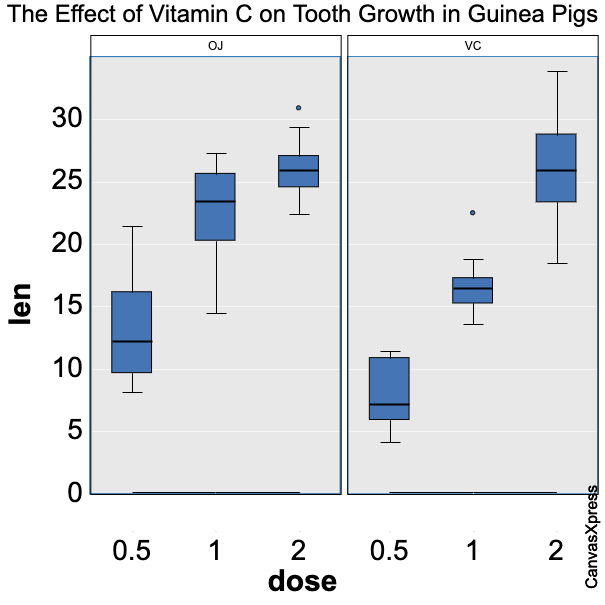
\includegraphics{boxplot_grouped_by_dosage.png}

\hypertarget{chart-events}{%
\subsection{Chart Events}\label{chart-events}}

CanvasXpress supports JavaScript events, with a default event handler
provided to display tooltip information on various aspects of a chart.
For example, in a basic bar chart the tooltip will display the variable
and sample labels plus intersecting value when the mouse however over a
bar.

CanvasXpress for Python supports the creation of custom events using a
\texttt{CXEvent} object:

\begin{Shaded}
\begin{Highlighting}[]
\ImportTok{from}\NormalTok{ canvasxpress.js.function }\ImportTok{import}\NormalTok{ CXEvent}

\NormalTok{CXEvent(}
    \BuiltInTok{id}\OperatorTok{=}\StringTok{"mousemove"}\NormalTok{,}
\NormalTok{    script}\OperatorTok{=}\StringTok{"t.showInfoSpan(e, \textquotesingle{}\textless{}pre\textgreater{}\textquotesingle{} + t.prettyJSON(o) + \textquotesingle{}\textless{}/pre\textgreater{}\textquotesingle{});"}\NormalTok{,}
\NormalTok{)}
\end{Highlighting}
\end{Shaded}

\texttt{id} is the name of the JavaScript event that will trigger the
logic. \texttt{script} is the content of the event function to be used
by CanvasXpress.

CanvasXpress provides each event function with three parameters:

\begin{itemize}
\tightlist
\item
  \texttt{o} is the data provided to the CanvasXpress chart
\item
  \texttt{e} is the JavaScript object for the triggering event
\item
  \texttt{t} is the full JavaScript CanvasXpress object (e.g., including
  the configuration)
\end{itemize}

Events are added to CanvasXpress for Python objects using a list of
events:

\begin{Shaded}
\begin{Highlighting}[]
\ImportTok{from}\NormalTok{ canvasxpress.canvas }\ImportTok{import}\NormalTok{ CanvasXpress}
\ImportTok{from}\NormalTok{ canvasxpress.render.jupyter }\ImportTok{import}\NormalTok{ CXNoteBook}
\ImportTok{from}\NormalTok{ canvasxpress.js.function }\ImportTok{import}\NormalTok{ CXEvent}

\NormalTok{cx }\OperatorTok{=}\NormalTok{ CanvasXpress(}
\NormalTok{    render\_to}\OperatorTok{=}\StringTok{"bar2"}\NormalTok{,}
\NormalTok{    data}\OperatorTok{=}\NormalTok{\{}
        \StringTok{"y"}\NormalTok{: \{}
            \StringTok{"vars"}\NormalTok{: [}\StringTok{"V1"}\NormalTok{],}
            \StringTok{"smps"}\NormalTok{: [}\StringTok{"S1"}\NormalTok{, }\StringTok{"S2"}\NormalTok{, }\StringTok{"S3"}\NormalTok{],}
            \StringTok{"data"}\NormalTok{: [[}\DecValTok{33}\NormalTok{, }\DecValTok{44}\NormalTok{, }\DecValTok{55}\NormalTok{]],}
\NormalTok{        \}}
\NormalTok{    \},}
\NormalTok{    config}\OperatorTok{=}\NormalTok{\{}
        \StringTok{"graphOrientation"}\NormalTok{: }\StringTok{"vertical"}\NormalTok{,}
        \StringTok{"plotBox"}\NormalTok{: }\VariableTok{True}\NormalTok{,}
        \StringTok{"showLegend"}\NormalTok{: }\VariableTok{False}\NormalTok{,}
        \StringTok{"smpLabelRotate"}\NormalTok{: }\DecValTok{90}\NormalTok{,}
        \StringTok{"smpTitle"}\NormalTok{: }\StringTok{"Samples"}\NormalTok{,}
        \StringTok{"theme"}\NormalTok{: }\StringTok{"CanvasXpress"}\NormalTok{,}
        \StringTok{"title"}\NormalTok{: }\StringTok{"Chart with Custom Event Showing X{-}Y Coordinates"}\NormalTok{,}
        \StringTok{"xAxis"}\NormalTok{: [}\StringTok{"V1"}\NormalTok{],}
        \StringTok{"xAxisTitle"}\NormalTok{: }\StringTok{"Value"}\NormalTok{,}
        \StringTok{"graphType"}\NormalTok{: }\StringTok{"Bar"}\NormalTok{,}
\NormalTok{    \},}
\NormalTok{    events}\OperatorTok{=}\NormalTok{[}
\NormalTok{        CXEvent(}
            \BuiltInTok{id}\OperatorTok{=}\StringTok{"mousemove"}\NormalTok{,}
\NormalTok{            script}\OperatorTok{=}\StringTok{"t.showInfoSpan(e, \textquotesingle{}\textless{}pre\textgreater{}X: \textquotesingle{} + e.clientX + \textquotesingle{}\textless{}br\textgreater{}Y: \textquotesingle{} + e.clientY + \textquotesingle{}\textless{}/pre\textgreater{}\textquotesingle{});"}\NormalTok{,}
\NormalTok{        ),}
\NormalTok{    ],}
\NormalTok{    width}\OperatorTok{=}\DecValTok{500}\NormalTok{,}
\NormalTok{    height}\OperatorTok{=}\DecValTok{500}\NormalTok{,}
\NormalTok{)}

\NormalTok{display }\OperatorTok{=}\NormalTok{ CXNoteBook(cx)}
\NormalTok{display.render()}
\end{Highlighting}
\end{Shaded}

\begin{verbatim}
<IPython.core.display.HTML object>
\end{verbatim}

\begin{verbatim}
<IPython.core.display.HTML object>
\end{verbatim}

\hypertarget{obtaining-example-code-from-any-canvasxpress-chart}{%
\subsection{Obtaining Example Code from Any CanvasXpress
Chart}\label{obtaining-example-code-from-any-canvasxpress-chart}}

CanvasXpress charts track their JSON data and configuration objects over
their lifespan, and they can convert attributes such as those into code
examples. On any CanvasXpress chart, such as the
\href{https://canvasxpress.org/examples/area-1.html}{examples at
CanvasXpress.org}, the right-click menu or configuration tool can be
used to obtain code in one of the supported languages:

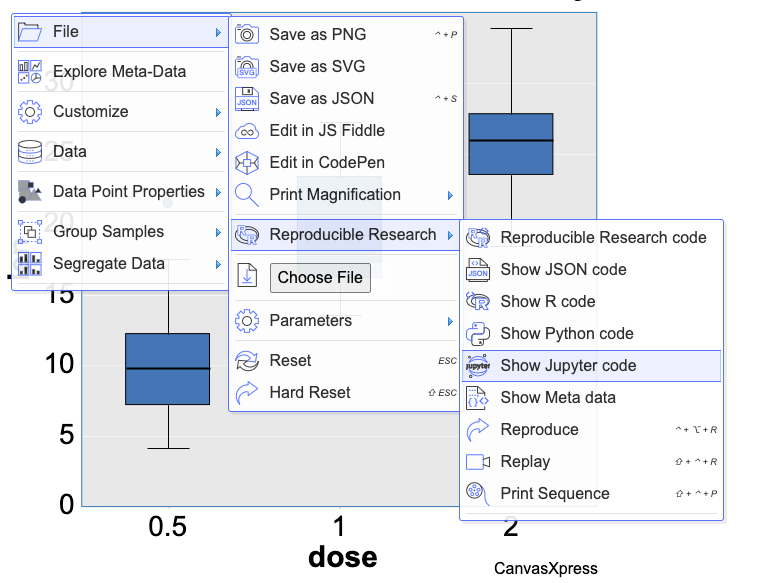
\includegraphics{reproducible_code_example.png}

Selecting the menu option will bring up a code sample that captures the
chart as currently configured. The best part about this feature is that
a chart can be customized using menu or configuration tool selections
and the code for the resultant chart can be captured, which is an
excellent way to learn about the many options available for chart
customization.

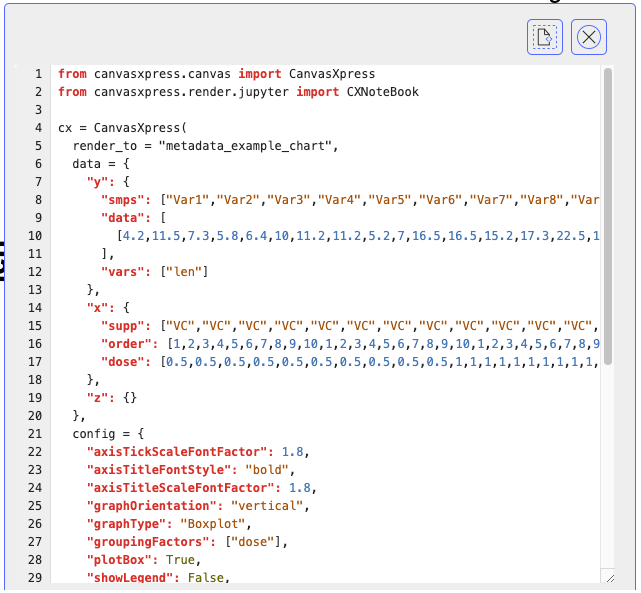
\includegraphics{reproducible_code.png}

CanvasXpress currently supports Python code examples for a local
development context with a pop-up browser and a Jupyter Notebook
context. However, remember that using a chart configuration in another
context, such as Streamlit, simply requires the use of the proper render
object.

\hypertarget{conclusion}{%
\subsection{Conclusion}\label{conclusion}}

CanvasXpress is a powerful and performant charting library with first
class support for data exploration. For many scientific and business
contexts, the ability to provide users with curated visualizations that
can be further enhanced or explored by the user is a game changing
capability that is sure to make solutions stand out from the crowd. We
have enjoyed using CanvasXpress in our own client work, and we are proud
to bring this excellent framework to the Python community for everyone
to enjoy. This introduction provides a comprehensive overview of chart
creation using Python, but be sure to visit the
\href{https://canvasxpress.org}{CanvasXpress site} to review the more
than 50 types of charts and the numerous examples providing inspiration
for each. Also be sure to check out our
\href{https://pypi.org/project/canvasxpress/}{PyPI page} for more
information on how to adopt CanvasXpress into your own projects and
experiments.



\end{document}
